\usepackage{tikz}\section{Visualizing Particle Generations with Color-Coded Knot Taxonomy}

To assist in publication clarity and pedagogical communication of the Vortex Æther Model (VAM), we introduce a color-coded, generation-labelled knot diagram aligned with particle taxonomy.

\subsection{Design Rationale}

Each particle is associated with a specific vortex knot type. We classify these into generations and quantum properties using a visual matrix:

\begin{itemize}
    \item \textbf{Rows} represent particle generations (1st, 2nd, 3rd).
    \item \textbf{Columns} represent particle classes (leptons, quarks, bosons).
    \item \textbf{Colors} encode linking number $Lk$: blue (low), green (moderate), red (high).
    \item \textbf{Symbols} show spin: trefoil loops for spin-1/2, twisted rings for spin-1.
\end{itemize}

\subsection{TikZ Illustration Template (for Future Rendering)}

\begin{figure}[h!]
    \centering
    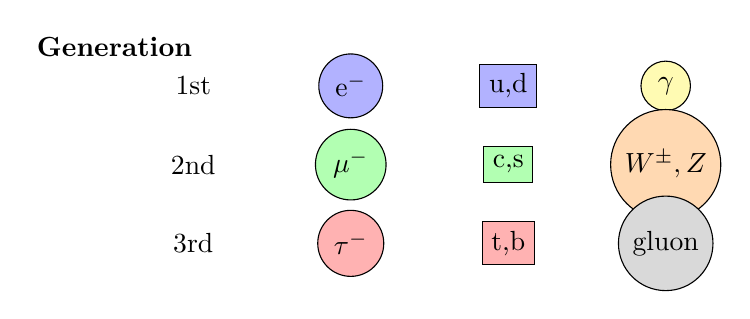
\begin{tikzpicture}[scale=1.0]
% Grid Labels
        \node at (0,3) {\textbf{Generation}};
        \node at (1,2.5) {1st};
        \node at (1,1.5) {2nd};
        \node at (1,0.5) {3rd};

% Leptons
        \node[draw,circle,fill=blue!30] at (3,2.5) {e$^-$};
        \node[draw,circle,fill=green!30] at (3,1.5) {$\mu^-$};
        \node[draw,circle,fill=red!30] at (3,0.5) {$\tau^-$};

% Quarks
        \node[draw,rectangle,fill=blue!30] at (5,2.5) {u,d};
        \node[draw,rectangle,fill=green!30] at (5,1.5) {c,s};
        \node[draw,rectangle,fill=red!30] at (5,0.5) {t,b};

% Bosons
        \node[draw,circle,fill=yellow!30] at (7,2.5) {$\gamma$};
        \node[draw,circle,fill=orange!30] at (7,1.5) {$W^\pm, Z$};
        \node[draw,circle,fill=gray!30] at (7,0.5) {gluon};

    \end{tikzpicture}
    \caption{Color-coded matrix of vortex-particle correspondences in VAM. Knot types and linking number are encoded in shape and fill.}
\end{figure}

This diagram helps communicate:
\begin{itemize}
    \item Generational hierarchy by vertical alignment
    \item Topological complexity by color intensity
    \item Physical role by shape (fermions vs. bosons)
\end{itemize}

\textbf{Note:} A full 3D knot rendering could be appended for each node, generated using knot plotting libraries like KnotPlot or Blender scripts.